\documentclass[12pt]{article}
\usepackage{float}
\usepackage{graphicx}
\usepackage[font=small,labelfont=bf]{caption}

\pagestyle{empty}
\setcounter{tocdepth}{4}
\setcounter{secnumdepth}{4}

\topmargin=0cm
\oddsidemargin=0cm
\textheight=22.0cm
\textwidth=16cm
\parindent=0cm
\parskip=0.15cm
\topskip=0truecm
\raggedbottom
\abovedisplayskip=3mm
\belowdisplayskip=3mm
\abovedisplayshortskip=0mm
\belowdisplayshortskip=2mm
\normalbaselineskip=12pt
\normalbaselines

\begin{document}

\vspace*{0.5in}
\centerline{\bf\Large Design Document - Iteration 2}

\vspace*{0.5in}
\centerline{\bf\Large Team PA-PI-a}

\vspace*{0.5in}
\centerline{\bf\Large 18 March 2018}

\vspace*{1.5in}
\begin{table}[htbp]
\caption{Team}
\begin{center}
\begin{tabular}{|r | c|}
\hline
Name & ID Number \\
\hline\hline
Melanie Taing & 40009850 \\
Laurie Gagnon & 22943433 \\
Wayne Yiel Leung & 26586988 \\
Jordan Rutty & 27300107 \\
Alice Barkhouse & 27486782 \\
Michael Foo & 40000225 \\
Pierre-Andre Leger & 40004010 \\
Colin Greczkowski & 40001600 \\
\hline
\end{tabular}
\end{center}
\end{table}

\clearpage

\tableofcontents

\clearpage

\section{Introduction}
\textit {From the template (delete me) --- The introduction of the document provides an overview of the entire document, briefly introducing what are its goals, and what information is to be found in it.}

\section{Architectural Design} \label{sec:arch}

\textit {From the template (delete me) --- This section must give a high-level description of the system in terms of its modules and their respective purpose and exact interfaces.}

\subsection{Architectural Diagram}

\textit {From the template (delete me) --- A UML class diagram or package diagram depicting the high-level structure of the system, accompanied by a one-paragraph text describing the rationale of this design. It is mandatory that the system be divided into at least two subsystems, and that the purpose of each of these subsystems be exposed here.}

\subsection{Subsystem Interface Specifications}

\textit {From the template (delete me) --- Specification of the software interfaces between the subsystems, i.e. specific messages (or function calls) that are exchanged by the subsystems. These are also often called ``Module Interface Specifications''.
Description of the parameters to be passed into these function calls in order to have a service fulfilled, including valid and invalid ranges of values. Each subsystem interface must be presented in a separate subsection.}

\section{Detailed Design} \label{sec:detail}

\textit {From the template (delete me) --- Complete description of the system design, describing one subsystem separately in respective subsection. UML class diagrams are to be used, as well as a short textual description describing the purpose of each class.}

\subsection{Subsystem X}

\subsubsection{Detailed Design Diagram}

\textit {From the template (delete me) --- UML class diagram depicting the internal structure of the subsystem, accompanied by a paragraph of text describing the rationale of this design.}

\subsubsection{Units Description}


\paragraph {AbstractAppController.java}
\begin{center}
\footnotesize
\begin{tabular}{|l|l|}
\hline
\textbf{Class Name }   & {AbstractAppController.java} \\ \hline
\textbf {Inherits} & {~} \\ \hline
\textbf {Description}   & {Abstract App Controller} \\ \hline
\textbf {Attributes} & ~ \\ \hline
\textbf {Methods} & 

\footnotesize
\begin{tabular}{l|l|l|l}
\textbf{Visibility} & \textbf{Method Name} & \textbf{Return type} &\textbf{Description} \\ \hline
public &AbstractAppController &~&Constructor\\ \hline
public &start &void &Abstract start class\\ \hline
public &shutdown&void &Abstract shutdown class\\ \hline
public &run &void &Abstract run class\\
\end{tabular} \\ \hline

\end{tabular}
\end{center}

\paragraph {AbstractEventListener.java}
\begin{center}
\footnotesize
\begin{tabular}{|l|l|}
\hline
\textbf {Class Name} & {AbstractEventListener.java} \\ \hline 
\textbf {Inherits} & { java.awt.event.ActionListener} \\ \hline 
\textbf {Description} & { Abstract Event Listener} \\ \hline 
\textbf {Attributes} &

\footnotesize
\begin{tabular}{l|l|l|l}
\textbf{Visibility} & \textbf{Data type} & \textbf{Name} & \textbf{Description} \\ \hline
package& AbstractView & view & ~  \\ \hline
package & AbstractViewController & controller & ~
\end{tabular} \\ \hline
\textbf {Methods} &

\footnotesize
\begin{tabular}{l|l|l|p{3.0cm}}
\vspace*{0.1cm}
\textbf{Visibility} & \textbf{Method Name} & \textbf{Return type} &\textbf{Description} \\ \hline
public &AbstractEventListener&~ &Constructor \\ \hline 
public &setView &void&Setter for view \\ \hline 
public &getView &AbstractView &Getter for view \\ \hline 
public&setController &void&Setter for controller \\ \hline 
public &getController&AbstractViewController&Getter for controller \\ \hline 
public &actionPerformed&void&Default message to implement this method in the view controller

\end{tabular} \\ \hline

\end{tabular}
\end{center}

\paragraph {AbstractModel.java}
\begin{center}
\footnotesize
\begin{tabular}{|l|l|}
\hline
\textbf {Class Name} & {AbstractModel.java} \\ \hline 
\textbf {Inherits} & {} \\ \hline 
\textbf {Description} & { Abstract class for models} \\ \hline 
\textbf {Attributes} &

\footnotesize
\begin{tabular}{l|l|l|l}
\textbf{Visibility} & \textbf{Data type} & \textbf{Name} & \textbf{Description} \\ \hline
package&boolean &boolNew&used to determine if id has been set \\ \hline
private & HashSet\textless AbstractView\textgreater & m\textunderscore views & stores the views \\
\end{tabular} \\ \hline
\textbf {Methods} &

\footnotesize
\begin{tabular}{l|l|l|l}
\textbf{Visibility} & \textbf{Method Name} & \textbf{Return type} &\textbf{Description} \\ \hline
public &isNew&boolean &getter for boolNew \\ \hline 
public &setIsNewModel&void&setter for boolNew \\ \hline 
public &setView &void &setter for views \\ \hline 
public &removeView &void &deletes views \\ \hline 
public &notifyViews&void &calls for update on all views
\end{tabular} \\ \hline

\end{tabular}
\end{center}

\paragraph {AbstractView.java}
\begin{center}
\footnotesize
\begin{tabular}{|l|l|}
\hline
\textbf {Class Name} & {AbstractView.java} \\ \hline 
\textbf {Inherits} & {} \\ \hline 
\textbf {Description} & { Abstract view class} \\ \hline 
\textbf {Attributes} & ~ \\ \hline
\textbf {Methods} &

\footnotesize
\begin{tabular}{l|l|l|l}
\textbf{Visibility} & \textbf{Method Name} & \textbf{Return type} &\textbf{Description} \\ \hline
package&AbstractView &Constructor \\ \hline 
public&update &void&abstract update class
\end{tabular} \\ \hline

\end{tabular}
\end{center}
\paragraph {AbstractViewController.java}
\begin{center}
\footnotesize
\begin{tabular}{|l|l|}
\hline
\textbf {Class Name} & {AbstractViewController.java} \\ \hline 
\textbf {Inherits} & {} \\ \hline 
\textbf {Description} & { Abstract class for view controller} \\ \hline 
\textbf {Attributes} &

\footnotesize
\begin{tabular}{l|l|l|p{5.8cm}}
\textbf{Visibility} & \textbf{Data type} & \textbf{Name} & \textbf{Description} \\ \hline
package &AbstractView &view &primary view \\ \hline 
package &AbstractView &secondaryView&secondary view \\ \hline 
private &boolean &controllerInitialized&determines if the controller has been initialized
\end{tabular} \\ \hline
\textbf {Methods} &

\footnotesize
\begin{tabular}{l|l|l|l}
\textbf{Visibility} & \textbf{Method Name} & \textbf{Return type} &\textbf{Description} \\ \hline
public&AbstractViewController&~&constructor \\ \hline 
public&setView&void&Setter for view \\ \hline 
public&getView&AbstractView &Getter for view \\ \hline 
public&setSecondaryView&void&Setter for secondary view \\ \hline 
public&getSecondaryView&AbstractView &Getter for secondary view \\ \hline 
public&setIsInitialized&void&Setter for controllerInitialized \\ \hline 
public&getIsInitialized&boolean&getter for controllerInitialized
\end{tabular} \\ \hline

\end{tabular}
\end{center}
\paragraph {AccountController.java}
\begin{center}
\footnotesize
\begin{tabular}{|l|l|}
\hline
\textbf {Class Name} & {AccountController.java} \\ \hline 
\textbf {Inherits} & { AbstractViewController} \\ \hline 
\textbf {Description} & { Controller for the accounts, initializing all the form elements associated to account} \\ \hline 
\textbf {Attributes} &

\footnotesize
\begin{tabular}{l|l|l|l}
\textbf{Visibility} & \textbf{Data type} & \textbf{Name} & \textbf{Description} \\ \hline
private &UserModel&user &user model object
\end{tabular} \\ \hline
\textbf {Methods} &

\footnotesize
\begin{tabular}{l|l|l|p{3cm}}
\textbf{Visibility} & \textbf{Method Name} & \textbf{Return type} &\textbf{Description} \\ \hline
protected&AccountController &~&Constructor \\ \hline 
protected &initController &void&binds event listeners/controls to all account view elements and populates form data \\ \hline 
public &setUser &void &setter for user \\ \hline 
public &getUser &UserModel &getter for user \\ \hline 
private &addButton &void &Behaviour of the "add account" button \\ \hline 
private &updateButton&void &Behaviour of the "update account" button \\ \hline 
private &deleteButton &void &Behaviour of the "delete account" button \\ \hline 
private &clearButton &void &Behaviour of the "clear" button \\ \hline 
protected &getAccountDataFromAddAccountInput&AccountModel&add data inputs to account model \\ \hline 
private &resetAddAccountInput &void &clear the UI account inputs \\ \hline 
public &getAccountDataFromRow&AccountModel&Given a row number, get account data \\ \hline 
protected &updateDataRowFromModel&void &modify account data given UI input \\ \hline 
public &update &void &Update the attached models
\end{tabular} \\ \hline

\end{tabular}
\end{center}


\paragraph {AccountModel.java}
\begin{center}
\footnotesize
\begin{tabular}{|l|l|}
\hline
\textbf {Class Name} & {AccountModel.java} \\ \hline 
\textbf {Inherits} & { AbstractModel} \\ \hline 
\textbf {Description} & { Model for bank accounts} \\ \hline 
\textbf {Attributes} &

\footnotesize
\begin{tabular}{l|p{3cm}|l|p{6cm}}
\textbf{Visibility} & \textbf{Data type} & \textbf{Name} & \textbf{Description} \\ \hline
private&int &accountId &the Id of the account \\ \hline 
private&String &bankName &the name of the bank the account is held with \\ \hline 
private&String &nickName &the nickname for the account \\ \hline 
private&int &balance &the dollar balance of the account \\ \hline 
package &AccountTransaction-\newline Repository&transactionsRepo &repository that holds account transaction information
\end{tabular} \\ \hline
\textbf {Methods} &

\footnotesize
\begin{tabular}{l|p{3.5cm}|p{3.5cm}|p{4.5cm}}
\textbf{Visibility} & \textbf{Method Name} & \textbf{Return type} &\textbf{Description} \\ \hline
public &AccountModel &Constructor\\ \hline 
public &hasId &boolean &determines if an account has an Id\\ \hline 
public &getId &int &getter for Id\\ \hline 
public &setId &void &setter for Id\\ \hline 
public &hasBankName&boolean &determines if an account has a bank name\\ \hline 
public &getBankName&String &getter for bank name\\ \hline 
public &setBankName &void &setter for bank name\\ \hline 
public &hasNickName&boolean &determines if an account has a nick name\\ \hline 
public &getNickName&String &getter for nick name\\ \hline 
public &setNickName &void &setter for nick name\\ \hline 
public &hasBalance&boolean &determines if an account has a balance\\ \hline 
public &getBalance&int &getter for balance\\ \hline 
public &setBalance&void &setter for balance\\ \hline 
public &toString &String &generates a formatted output of all the account details\\ \hline 
public &setAccount-\newline TransactionRepository&void &Setter for transactionsRepo\\ \hline 
public &getAccount-\newline TransactionRepository&AccountTransaction-\newline Repository &Getter for transactionsRepo\\ \hline 
public &getMapOf-\newline AllTransactions &TransactionMap&gets map of all transactions\\ \hline 
public &getListOfAll-\newline Transactions &TransactionList&gets list of all transactions\\ \hline 
public &saveTransaction&void &Saves a transaction to the repository\\ \hline 
public &deleteTransaction&void &deletes a transaction from the repository
\end{tabular} \\ \hline

\end{tabular}
\end{center}
\paragraph {AccountRepository.java}
\begin{center}
\footnotesize
\begin{tabular}{|l|l|}
\hline
\textbf {Class Name} & {AccountRepository.java} \\ \hline 
\textbf {Inherits} & {} \\ \hline 
\textbf {Description} & { Provides functionality to a user's bank accounts database} \\ \hline 
\textbf {Attributes} &

\footnotesize
\begin{tabular}{l|l|l|l}
\textbf{Visibility} & \textbf{Data type} & \textbf{Name} & \textbf{Description} \\ \hline
package&Database &myDatabase &Database that stores account information\\ \hline 
package&SQLStringFactory &sql &Builds valid SQL statements\\ \hline 
package &String &tableName &Name of the table\\ \hline 
package &String &primaryKey &Name of the databases' primary key\\ \hline 
package &Boolean &boolAllLoaded &Have all accounts been loaded in database?\\ \hline 
package &AccountMap &itemMap&holds loaded account models
\end{tabular} \\ \hline
\textbf {Methods} &

\footnotesize
\begin{tabular}{l|l|l|l}
\textbf{Visibility} & \textbf{Method Name} & \textbf{Return type} &\textbf{Description} \\ \hline
public &AccountRepository &~&Constructor\\ \hline 
protected &hasItemCached&boolean &checks if item is in itemMap\\ \hline 
public &saveItem&void &Save or update an account\\ \hline 
public&deleteItem&void&Deletes an account\\ \hline 
public &getItem&AccountModel&getter for account item\\ \hline 
public &getMapOfAllItems&AccountMap&getter for map of all items\\ \hline 
public&getListOfAllItems&AccountList&getter for all items\\ \hline 
protected &loadItem&void&load an account\\ \hline 
protected&loadAll&void&load all accounts\\ \hline 
protected&setItemFromResult&void&populate the model with account information\\ \hline 
protected&addItemToMap&void&Add an account to the item map
\end{tabular} \\ \hline

\end{tabular}
\end{center}
\paragraph {AccountTransactionRepository.java}
\begin{center}
\footnotesize
\begin{tabular}{|l|l|}
\hline
\textbf {Class Name} & {AccountTransactionRepository.java} \\ \hline 
\textbf {Inherits} & { TransactionRepository} \\ \hline 
\textbf {Description} & { Contains access to all of the transactions for an account} \\ \hline 
\textbf {Attributes} &

\footnotesize
\begin{tabular}{l|l|l|p{8cm}}
\textbf{Visibility} & \textbf{Data type} & \textbf{Name} & \textbf{Description} \\ \hline
package&AccountModel&account &The account object from which we are accessing transactions
\end{tabular} \\ \hline
\textbf {Methods} &

\footnotesize
\begin{tabular}{l|p{3.5cm}|l|l}
\textbf{Visibility} & \textbf{Method Name} & \textbf{Return type} &\textbf{Description} \\ \hline
public&AccountTransaction-\newline Repository&~&Constructor\\ \hline 
public&setAccount&void&Setter for account\\ \hline 
public&getAccount&AccountModel&Getter for account\\ \hline 
public&hasAccount&boolean &Check if account has been initialized\\ \hline 
public &loadAllItems&void&load all transactions for account\\ \hline 
public &saveItem&void&Save a transaction to account
\end{tabular} \\ \hline

\end{tabular}
\end{center}
\paragraph {AccountView.java}
\begin{center}
\footnotesize
\begin{tabular}{|l|l|}
\hline
\textbf {Class Name} & {AccountView.java} \\ \hline 
\textbf {Inherits} & { AbstractView} \\ \hline 
\textbf {Description} & { The view for accounts (accounts UI)} \\ \hline 
\textbf {Attributes} &

\footnotesize
\begin{tabular}{l|l|l|l}
\textbf{Visibility} & \textbf{Data type} & \textbf{Name} & \textbf{Description} \\ \hline
private &JPanel &panel&Various account UI elements\\ \hline 
private &DefaultTableModel &model &...\\ \hline 
private &JLabel &accLabel\\ \hline 
private &JLabel &accountIDLabel\\ \hline 
private &JLabel &bankLabel\\ \hline 
private &JLabel &nicknameLabel\\ \hline 
private &JLabel &balanceLabel\\ \hline 
private &JButton &addButton\\ \hline 
private &JButton &updateButton\\ \hline 
private &JButton &deleteButton\\ \hline 
private &JButton &clearButton\\ \hline 
private &JTextField &accountIDTextfield\\ \hline 
private &JTextField &bankTextfield\\ \hline 
private &JTextField &nicknameTextfield\\ \hline 
private &JTextField &balanceTextfield\\ \hline 
private &JTable &table\\ \hline 
private &JScrollPane &scrollPane&
\end{tabular} \\ \hline

\end{tabular}
\end{center}
\begin{center}
\footnotesize
\begin{tabular}{|l|l|}
\hline
\textbf {Methods} &

\footnotesize
\begin{tabular}{l|l|l|p{5cm}}
\textbf{Visibility} & \textbf{Method Name} & \textbf{Return type} &\textbf{Description} \\ \hline
public  &getPanel&JPanel&getter for panel\\ \hline 
public  &setPanel&void&setter for panel\\ \hline 
public  &getTableModel&DefaultTableModel&getter for table model\\ \hline 
public  &setTableModel&void&setter for table model\\ \hline 
public  &getAccLabel&JLabel&getter for account label\\ \hline 
public  &setAccLabel&void&setter for account label\\ \hline 
public  &getAccountIDLabel&JLabel&getter for account id label\\ \hline 
public  &setAccountIDLabel&void&setter getter account id label\\ \hline 
public  &getBankLabel&JLabel&getter for bank label\\ \hline 
public  &setBankLabel&void&setter for bank label\\ \hline 
public  &getNicknameLabel&JLabel&getter for nickname label\\ \hline 
public  &setNickname&void&setter for nickname label\\ \hline 
public  &getBalanceLabel&JLabel&getter for balance label\\ \hline 
public  &setBalanceLabel&void&setter for balance label\\ \hline 
public  &getAccountIDTextfield&JTextField&getter for account id textfield\\ \hline 
public  &setAccountIDTextfield&void&setter for account id textfield\\ \hline 
public  &getBankTextfield&JTextField&getter for bank textfield\\ \hline 
public  &setBankTextfield&void&setter for bank textfield\\ \hline 
public  &getNicknameTextfield&JTextField&getter for nickname textfield\\ \hline 
public  &setNicknameTextfield&void&setter for nickname textfield\\ \hline 
public  &getBalanceTextfield&JTextField&getter for balance textfield\\ \hline 
public  &setBalanceTextfield&void&setter for balance textfield\\ \hline 
public  &getAddButton&Button&getter for add button\\ \hline 
public  &setAddButton&void&setter for add button\\ \hline 
public  &getUpdateButton&JButton&getter for update button\\ \hline 
public  &setUpdateButton&void&setter for update button\\ \hline 
public  &getDeleteButton&JButton&getter for delete button\\ \hline 
public  &setDeleteButton&void&setter for delete button\\ \hline 
public  &getClearButton&JButton&getter for clear button\\ \hline 
public  &setClearButton&void&setter for clear button\\ \hline 
public  &getTable&JTable&getter for table\\ \hline 
public  &setTable&void&setter for table\\ \hline 
public  &getScrollPane&JScrollPane&getter for scroll pane\\ \hline 
public  &setScrollPane&void&setter for scroll pane\\ \hline 
public &update &void &updates the Jtable\\ \hline 
private &createAccPanel &void &creates the account UI elements\\ \hline 
private &setLayout &void &sets the visuals and grouping of the UI layout
\end{tabular} \\ \hline

\end{tabular}
\end{center}
\paragraph {Database.java}
\begin{center}
\footnotesize
\begin{tabular}{|l|l|}
\hline
\textbf {Class Name} & {Database.java} \\ \hline 
\textbf {Inherits} & {} \\ \hline 
\textbf {Description} & { The database object for storing/retrieving/altering data in the various databases.} \\ \hline 
\textbf {Attributes} &

\footnotesize
\begin{tabular}{l|l|l|l}
\textbf{Visibility} & \textbf{Data type} & \textbf{Name} & \textbf{Description} \\ \hline
private&String &m\textunderscore driver& database driver\\ \hline 
private&String &m\textunderscore dbName& database name\\ \hline 
private&Connection &m\textunderscore connection& connection to database
\end{tabular} \\ \hline
\textbf {Methods} &

\footnotesize
\begin{tabular}{l|l|l|l}
\textbf{Visibility} & \textbf{Method Name} & \textbf{Return type} &\textbf{Description} \\ \hline
public&Database &    &Constructor\\ \hline 
public&getConnection &Connection &Getter for connection\\ \hline 
public&fetchSQL&ResultSet &Executes an SQL query\\ \hline 
public &updateSQL &Integer &Executes an SQL update\\ \hline 
public &shutdown&void&Terminates connection
\end{tabular} \\ \hline

\end{tabular}
\end{center}
\paragraph {DummyAppController.java}
\begin{center}
\footnotesize
\begin{tabular}{|l|l|}
\hline
\textbf {Class Name} & {DummyAppController.java} \\ \hline 
\textbf {Inherits} & { AbstractAppController} \\ \hline 
\textbf {Description} & { Controller for a dummy app} \\ \hline 
\textbf {Attributes} &

\footnotesize
\begin{tabular}{l|l|l|l}
\textbf{Visibility} & \textbf{Data type} & \textbf{Name} & \textbf{Description} \\ \hline
package &Database &myDatabase &the database where app data is stored\\ \hline 
package&SQLStringFactory &sql &Builds valid SQL statements
\end{tabular} \\ \hline
\textbf {Methods} &

\footnotesize
\begin{tabular}{l|l|l|l}
\textbf{Visibility} & \textbf{Method Name} & \textbf{Return type} &\textbf{Description} \\ \hline
public &DummyAppController &~&Constructor\\ \hline 
public &start &void &starts the app\\ \hline 
public &run &void &initialize and run the dummy app
\end{tabular} \\ \hline

\end{tabular}
\end{center}
\paragraph {ImportTransaction.java}
\begin{center}
\footnotesize
\begin{tabular}{|l|l|}
\hline
\textbf {Class Name} & {ImportTransaction.java} \\ \hline 
\textbf {Inherits} & {} \\ \hline 
\textbf {Description} & { Imports transaction data from a CSV file} \\ \hline 
\textbf {Attributes} &

\footnotesize
\begin{tabular}{l|p{3cm}|p{3cm}|p{5.5cm}}
\textbf{Visibility} & \textbf{Data type} & \textbf{Name} & \textbf{Description} \\ \hline
package&String &transactionFilePath&the filepath of the csv that holds new transaction data\\ \hline 
private &AccountTransaction-\newline Repository &accountTransaction-\newline Repository &the repository that holds transaction data
\end{tabular} \\ \hline
\textbf {Methods} &

\footnotesize
\begin{tabular}{l|p{4cm}|l|p{5.5cm}}
\textbf{Visibility} & \textbf{Method Name} & \textbf{Return type} &\textbf{Description} \\ \hline
public &setAccount-\newline TransactionRepository&void&setter for accountTransactionRepository\\ \hline 
public&addTransaction&void &Imports transactions from CSV and stores in repository
\end{tabular} \\ \hline

\end{tabular}
\end{center}
\paragraph {Iteration2AppController.java}
\begin{center}
\footnotesize
\begin{tabular}{|l|l|}
\hline
\textbf {Class Name} & {Iteration2AppController.java} \\ \hline 
\textbf {Inherits} & {} \\ \hline 
\textbf {Description} & App controller for current project iteration \\ \hline 
\textbf {Attributes} &

\footnotesize
\begin{tabular}{l|l|l|p{4.5cm}}
\textbf{Visibility} & \textbf{Data type} & \textbf{Name} & \textbf{Description} \\ \hline
package &Database &myDatabase &the database where app data is stored\\ \hline 
package&SQLStringFactory &sql &Builds valid SQL statements\\ \hline 
package &AccountRepository &theAccountRespository&the repository that holds account data\\ \hline 
package &TransactionRepository &theTransactionRepository&the repository that holds transaction data
\end{tabular} \\ \hline
\textbf {Methods} &

\footnotesize
\begin{tabular}{l|l|l|p{6cm}}
\textbf{Visibility} & \textbf{Method Name} & \textbf{Return type} &\textbf{Description} \\ \hline
public &Iteration2AppController&~&Constructor\\ \hline 
public &start &void &starts the app\\ \hline 
protected&devStart &void &starts the app in development mode\\ \hline 
protected&productionStart &void &starts the app in production mode\\ \hline 
protected&InsertFakeAccounts &void &Adds some generic data to accounts repository for development\\ \hline 
public &run &void&initializes and runs the i2 app
\end{tabular} \\ \hline

\end{tabular}
\end{center}

\paragraph {MainController.java}
\begin{center}
\footnotesize
\begin{tabular}{|l|l|}
\hline
\textbf {Class Name} & {MainController.java} \\ \hline 
\textbf {Inherits} & { AbstractViewController} \\ \hline 
\textbf {Description} & { The main controller for the app} \\ \hline 
\textbf {Attributes} &

\footnotesize
\begin{tabular}{l|l|l|p{7cm}}
\textbf{Visibility} & \textbf{Data type} & \textbf{Name} & \textbf{Description} \\ \hline
package &UserModel &user &the user of the app
\end{tabular} \\ \hline
\textbf {Methods} &

\footnotesize
\begin{tabular}{l|l|l|p{6cm}}
\textbf{Visibility} & \textbf{Method Name} & \textbf{Return type} &\textbf{Description} \\ \hline
public &MainController &~&Constructor\\ \hline 
public &setUser &void &Setter for user\\ \hline 
public &getUser &UserModel &Getter for user\\ \hline 
public &initController &void &initialized the account, transaction and main view
\end{tabular} \\ \hline

\end{tabular}
\end{center}
\paragraph {MainView.java}
\begin{center}
\footnotesize
\begin{tabular}{|l|l|}
\hline
\textbf {Class Name} & {MainView.java} \\ \hline 
\textbf {Inherits} & { AbstractView} \\ \hline 
\textbf {Description} & { The main view for the app} \\ \hline 
\textbf {Attributes} &

\footnotesize
\begin{tabular}{l|l|l|l}
\textbf{Visibility} & \textbf{Data type} & \textbf{Name} & \textbf{Description} \\ \hline
protected &JFrame &mainFrame &Swing framework main frame to display the UI\\ \hline 
private &String &title &The title of the main view
\end{tabular} \\ \hline
\textbf {Methods} &

\footnotesize
\begin{tabular}{l|l|l|p{6cm}}
\textbf{Visibility} & \textbf{Method Name} & \textbf{Return type} &\textbf{Description} \\ \hline
public &MainView &~&constructor\\ \hline 
public &getFrame&JFrame &getter for mainFrame\\ \hline 
public &setFrame &void &setter for mainFrame\\ \hline 
public &update &void&refreshes the main frame\\ \hline 
public &display&void &creates the UI frame \\ \hline 
public&setLayout &void &populates the UI frame with various UI account elements
\end{tabular} \\ \hline

\end{tabular}
\end{center}
\paragraph {SQLStringFactory.java}
\begin{center}
\footnotesize
\begin{tabular}{|l|l|}
\hline
\textbf {Class Name} & {SQLStringFactory.java} \\ \hline 
\textbf {Inherits} & {} \\ \hline 
\textbf {Description} & { Builds formatted SQL statements for interaction with databases.} \\ \hline 
\textbf {Attributes} &

\footnotesize
\begin{tabular}{l|l|l|l}
\textbf{Visibility} & \textbf{Data type} & \textbf{Name} & \textbf{Description} \\ \hline
private &SQLStringFactory&m\textunderscore instance&holds the instance of the SQLStringFactory
\end{tabular} \\ \hline
\textbf {Methods} &

\footnotesize
\begin{tabular}{l|l|l|p{5cm}}
\textbf{Visibility} & \textbf{Method Name} & \textbf{Return type} &\textbf{Description} \\ \hline
public&getInstance&SQLStringFactory&getter for the instance of the SQLStringFactory\\ \hline 
private&SQLStringFactory&~&constructor\\ \hline 
public&deleteTable&String &Creates a drop table SQL statement\\ \hline 
public&createTable&String &Creates a create table SQL statement\\ \hline 
public&addColumn&String &Creates an alter table SQL statement\\ \hline 
public &addEntry&String &Creates an insert into SQL statement\\ \hline 
public &addEntryUsingMap&String &Creates an insert into SQL statement using mapped values\\ \hline 
public &updateEntryUsingMap&String &Creates an update SQL statement using mapped values\\ \hline 
public &selectEntryUsingMap&String &Creates a select SQL statement using mapped values\\ \hline 
protected &buildWhereCondition&String &Generates chunks of SQL where conditions\\ \hline 
protected &EscapeSQLValue&String &"Cleans" SQL statements to prevent injection\\ \hline 
public&showAll&String &Creates a basic select all SQL statement.
\end{tabular} \\ \hline

\end{tabular}
\end{center}
\paragraph {SQLValueMap.java}
\begin{center}
\footnotesize
\begin{tabular}{|l|l|}
\hline
\textbf {Class Name} & {SQLValueMap.java} \\ \hline 
\textbf {Inherits} & { LinkedHashMap\textless String,String\textgreater } \\ \hline 
\textbf {Description} & { Shortcut class to shorten the LinkedHashMap setter and eliminate the need to type cast} \\ \hline 
\textbf {Attributes} & \\ \hline
\textbf {Methods} &

\footnotesize
\begin{tabular}{l|l|l|l}
\textbf{Visibility} & \textbf{Method Name} & \textbf{Return type} &\textbf{Description} \\ \hline
public&put &void&put either float or integers as String
\end{tabular} \\ \hline

\end{tabular}
\end{center}
\paragraph {TransactionController.java}
\begin{center}
\footnotesize
\begin{tabular}{|l|l|}
\hline
\textbf {Class Name} & {TransactionController.java} \\ \hline 
\textbf {Inherits} & { AbstractViewController} \\ \hline 
\textbf {Description} & { Controller for the transactions, initializing all the form elements associated with transactions} \\ \hline 
\textbf {Attributes} &

\footnotesize
\begin{tabular}{l|l|l|l}
\textbf{Visibility} & \textbf{Data type} & \textbf{Name} & \textbf{Description} \\ \hline
private &UserModel&user &user model object\\ \hline 
package &int &accountIndex &the index of an account
\end{tabular} \\ \hline
\textbf {Methods} &

\footnotesize
\begin{tabular}{l|l|l|p{4cm}}
\textbf{Visibility} & \textbf{Method Name} & \textbf{Return type} &\textbf{Description} \\ \hline
protected&TransactionController &~&Constructor\\ \hline 
protected &initController &void&binds event listeners/controls to all transaction view elements and populates form data\\ \hline 
public &setUser &void&Setter for user\\ \hline 
public &getUser &UserModel &Getter for user\\ \hline 
private &addButton &void &Behaviour of the "add transaction" button\\ \hline 
private &deleteButton &void &Behaviour of the "delete transaction" button\\ \hline 
private &clearButton &void &Behaviour of the "clear" button\\ \hline 
private &importTransactionButton&void &Behaviour of the "import transaction" button\\ \hline 
protected &getTransactionDataFromRow&TransactionModel&Returns transaction data based on row number\\ \hline 
protected &getTransactionDataFromInput&TransactionModel&Returns transaction data based on UI input\\ \hline 
protected &updateDataRowFromModel&void &Updates a row in the transaction table based on UI input\\ \hline 
protected &getAccountDataFromRow&AccountModel&Gets the account data for the currently selected row\\ \hline 
public&update &void &Updates the attached models.
\end{tabular} \\ \hline

\end{tabular}
\end{center}

\paragraph {TransactionModel.java}
\begin{center}
\footnotesize
\begin{tabular}{|l|l|}
\hline
\textbf {Class Name} & {TransactionModel.java} \\ \hline 
\textbf {Inherits} & { AbstractModel} \\ \hline 
\textbf {Description} & { Model for the transactions} \\ \hline 
\textbf {Attributes} &

\footnotesize
\begin{tabular}{l|l|l|l}
\textbf{Visibility} & \textbf{Data type} & \textbf{Name} & \textbf{Description} \\ \hline
package &Integer&transactionId&id of a transaction\\ \hline 
package &Integer &accountId&id of an account\\ \hline 
package &String &type&type of transaction\\ \hline 
package &String &date&date of transaction\\ \hline 
package &Integer &amount&dollar amount of a transaction\\ \hline 
package &String  &description&text description of a transaction
\end{tabular} \\ \hline
\textbf {Methods} &

\footnotesize
\begin{tabular}{l|l|l|p{6cm}}
\textbf{Visibility} & \textbf{Method Name} & \textbf{Return type} &\textbf{Description} \\ \hline
public &TransactionModel&~&Constructor\\ \hline 
public &setId &void &setter for transactionId\\ \hline 
public &getId &Integer&getter for transactionId\\ \hline 
public &setAccountId &void &setter for accountId\\ \hline 
public &getAccountId &Integer&getter for accountId\\ \hline 
public &setType &void &setter for type\\ \hline 
public &getType &String &getter for type\\ \hline 
public &setDate &void &setter for date\\ \hline 
public &getDate &String &getter for date\\ \hline 
public &setAmount &void &setter for amount\\ \hline 
public &getAmount &Integer&getter for amount\\ \hline 
public &setDescription &void &setter for description\\ \hline 
public &getDescription &String &getter for description\\ \hline 
public &toString &String &generates a formatted output of all the transaction details
\end{tabular} \\ \hline

\end{tabular}
\end{center}
\paragraph {TransactionRepository.java}
\begin{center}
\footnotesize
\begin{tabular}{|l|l|}
\hline
\textbf {Class Name} & {TransactionRepository.java} \\ \hline 
\textbf {Inherits} & {} \\ \hline 
\textbf {Description} & { Contains access to all of the transactions on the system} \\ \hline 
\textbf {Attributes} &

\footnotesize
\begin{tabular}{l|p{4cm}|l|p{6cm}}
\textbf{Visibility} & \textbf{Data type} & \textbf{Name} & \textbf{Description} \\ \hline
package&SQLStringFactory&sql &Builds valid SQL statements\\ \hline 
package &Database &myDatabase&Database that stores transaction information\\ \hline 
package &HashMap\textless Integer, -\newline TransactionModel\textgreater &itemMap &Holds loaded account models\\ 
\end{tabular} \\ \hline
\textbf {Methods} &

\footnotesize
\begin{tabular}{l|l|l|p{6cm}}
\textbf{Visibility} & \textbf{Method Name} & \textbf{Return type} &\textbf{Description} \\ \hline
public&TransactionRepository&~&Constructor\\ \hline 
public &loadItem &void &load a transaction\\ \hline 
public &loadAllItems&void&load all transactions \\ \hline 
public &saveItem&void&Save a transaction to its account\\ \hline 
private &setFromResult &void &populate the model with a transaction result\\ \hline 
private &addToMap &void &Put a transaction in the itemMap

\end{tabular} \\ \hline

\end{tabular}
\end{center}
\paragraph {TransactionView.java}
\begin{center}
\footnotesize
\begin{tabular}{|l|l|}
\hline
\textbf {Class Name} & {TransactionView.java} \\ \hline 
\textbf {Inherits} & { AbstractView} \\ \hline 
\textbf {Description} & { The view for transactions (transaction UI)} \\ \hline 
\textbf {Attributes} &

\footnotesize
\begin{tabular}{l|l|l|l}
\textbf{Visibility} & \textbf{Data type} & \textbf{Name} & \textbf{Description} \\ \hline
private &JPanel &panel&Various account UI elements\\ \hline 
private &DefaultTableModel &model &...\\ \hline 
private &JLabel &accountIDLabel\\ \hline 
private &JLabel &transactionIDLabel\\ \hline 
private &JLabel &transLabel\\ \hline 
private &JLabel &typeLabel\\ \hline 
private &JLabel &dateLabel\\ \hline 
private &JLabel &amountLabel\\ \hline 
private &JLabel &descriptionLabel\\ \hline 
private &JButton &addButton\\ \hline 
private &JButton &updateButton\\ \hline 
private &JButton &deleteButton\\ \hline 
private &JButton &clearButton\\ \hline 
private &JButton &importButton\\ \hline 
private &JTextField &accountIDTextfield\\ \hline 
private &JTextField &transactionIDTextfield\\ \hline 
private &JTextField &typeTextfield\\ \hline 
private &JTextField &dateTextfield\\ \hline 
private &JTextField &amountTextfield\\ \hline 
private &JTextArea &descriptionTextArea\\ \hline 
private &JTable &table\\ \hline 
private &JScrollPane &scrollPane
\end{tabular} \\ \hline

\end{tabular}
\end{center}
\begin{center}
\footnotesize
\begin{tabular}{|l|l|}
\hline
\textbf {Methods} &

\footnotesize
\begin{tabular}{l|l|l|p{5cm}}
\textbf{Visibility} & \textbf{Method Name} & \textbf{Return type} &\textbf{Description} \\ \hline
public &TransactionView &~&Constructor\\ \hline 
public  &getPanel&JPanel&getter for panel\\ \hline 
public  &setPanel&void&setter for panel\\ \hline 
public  &getTableModel&DefaultTableModel&getter for table model\\ \hline 
public  &setTableModel&void&setter for table model\\ \hline 
public  &getAccountIDLabel&JLabel&getter for account id label\\ \hline 
public  &setAccountIDLabel&void&setter getter account id label\\ \hline 
public &setTransactionIDLabel&void&setter for TransactionIDLabel\\ \hline 
public &setTransLabel&void&setter for TransLabel\\ \hline 
public &setTypeLabel&void&setter for TypeLabel\\ \hline 
public &setDateLabel&void&setter for DateLabel\\ \hline 
public &setAmountLabel&void&setter for AmountLabe\\ \hline 
public &setDescriptionLabel&void&setter for DescriptionLabel\\ \hline 
public &setAccountIDTextfield&void&setter for AccountIDTextfield\\ \hline 
public &setTransactionIDTextfield&void&setter for TransactionIDTextfield\\ \hline 
public &setTypeTextfield&void&setter for TypeTextfield\\ \hline 
public &setDateTextfield&void&setter for DateTextfield\\ \hline 
public &setAmountTextfield&void&setter for AmountTextfield\\ \hline 
public &setDescriptionTextArea&void&setter for DescriptionTextArea\\ \hline 
public &getTransactionIDLabel&JLabel&getter for TransactionIDLabel\\ \hline 
public &getTransLabel &JLabel&getter for TransLabel\\ \hline 
public &getTypeLabel &JLabel&getter for TypeLabel\\ \hline 
public &getDateLabel &JLabel&getter for DateLabel\\ \hline 
public &getAmountLabel &JLabel&getter for AmountLabel\\ \hline 
public &getDescriptionLabel&JLabel&getter for DescriptionLabel\\ \hline 
public &getAccountIDTextfield&JTextField&getter for AccountIDTextfield\\ \hline 
public &getTransactionIDTextfield&JTextField&getter for TransactionIDTextfield\\ \hline 
public &getTypeTextfield&JTextField&getter for TypeTextfield\\ \hline 
public &getDateTextfield&JTextField&getter for DateTextfield\\ \hline 
public &getAmountTextfield&JTextField&getter for AmountTextfield\\ \hline 
public &getDescriptionTextArea&JTextArea&getter for DescriptionTextArea\\ \hline 
public  &getAddButton&Button&getter for add button\\ \hline 
public  &setAddButton&void&setter for add button\\ \hline 
public  &getUpdateButton&JButton&getter for update button\\ \hline 
public  &setUpdateButton&void&setter for update button\\ \hline 
public  &getDeleteButton&JButton&getter for delete button\\ \hline 
public  &setDeleteButton&void&setter for delete button\\ \hline 
public  &getClearButton&JButton&getter for clear button\\ \hline 
public  &setClearButton&void&setter for clear button\\ \hline 
public  &getImportButton&JButton&getter for import button\\ \hline 
public  &setImportButton&void&setter for import button\\ \hline 
public  &getTable&JTable&getter for table\\ \hline 
public  &setTable&void&setter for table\\ \hline 
public  &getScrollPane&JScrollPane&getter for scroll pane\\ \hline 
public  &setScrollPane&void&setter for scroll pane\\ \hline 
public &update &void &updates the Jtable\\ \hline 
private &createTransPanel&void &creates the transaction UI elements\\ \hline 
private &setLayout &void &sets the visuals and grouping of the UI layout
\end{tabular} \\ \hline


\end{tabular}
\end{center}
\paragraph {UserModel.java}
\begin{center}
\footnotesize
\begin{tabular}{|l|l|}
\hline
\textbf {Class Name} & {UserModel.java} \\ \hline 
\textbf {Inherits} & {} \\ \hline 
\textbf {Description} & { Model for the user of the app} \\ \hline 
\textbf {Attributes} &

\footnotesize
\begin{tabular}{l|l|l|l}
\textbf{Visibility} & \textbf{Data type} & \textbf{Name} & \textbf{Description} \\ \hline
package &AccountRepository &accountsRepo &the repository that holds account data
\end{tabular} \\ \hline
\textbf {Methods} &

\footnotesize
\begin{tabular}{l|l|l|p{5cm}}
\textbf{Visibility} & \textbf{Method Name} & \textbf{Return type} &\textbf{Description} \\ \hline
public&UserModel&~&Constructor\\ \hline 
public &getName &String &gets the user's name\\ \hline 
public &setAccountRepository&void &Setter for accounts Repo\\ \hline 
public &getAccountRepository&AccountRepository &Getter for accounts Repo\\ \hline 
public &getMapOfAllAccounts& AccountMap&gets map of all accounts\\ \hline 
public &getListOfAllAccounts& AccountList&gets list of all accounts\\ \hline 
public &saveAccount&void &Saves an account to the repository\\ \hline 
public &deleteAccount&void &deletes an account from the repository\\ \hline 
public &getAccountAtIndex &AccountModel &gets account based on row index number
\end{tabular} \\ \hline

\end{tabular}
\end{center}
\paragraph {Util.java}
\begin{center}
\footnotesize
\begin{tabular}{|l|l|}
\hline
\textbf {Class Name} & {Util.java} \\ \hline 
\textbf {Inherits} & {} \\ \hline 
\textbf {Description} & { Various tools used by the app} \\ \hline 
\textbf {Attributes} & ~ \\ \hline
\textbf {Methods} &

\footnotesize
\begin{tabular}{l|l|l|l}
\textbf{Visibility} & \textbf{Method Name} & \textbf{Return type} &\textbf{Description} \\ \hline
public &isNumeric &boolean &Check if a string is numeric
\end{tabular} \\ \hline

\end{tabular}
\end{center}

\section{Dynamic Design Scenarios}
To illustrate the interactions between the difference classes of our system, we have drawn sequence diagrams for the main features of our program. For simplicity, the repositories are the lowest layer of abstraction in the diagrams. We have also included a sequence diagram of the AccountRespository saving an account to the database using the Database class (Figure 2).
\newpage
\subsection{Adding an account}
After completing the text field and pressing the "add" button, the addButton method from the AccountController is triggered. The controller first gathers and validates the inputs. If the inputs are valid, the controller initializes an AccountModel object and constructs it using setters. The object is saved by calling the UserModel's saveAccount method, which in turn calls its AccountRepository's saveItem method. 
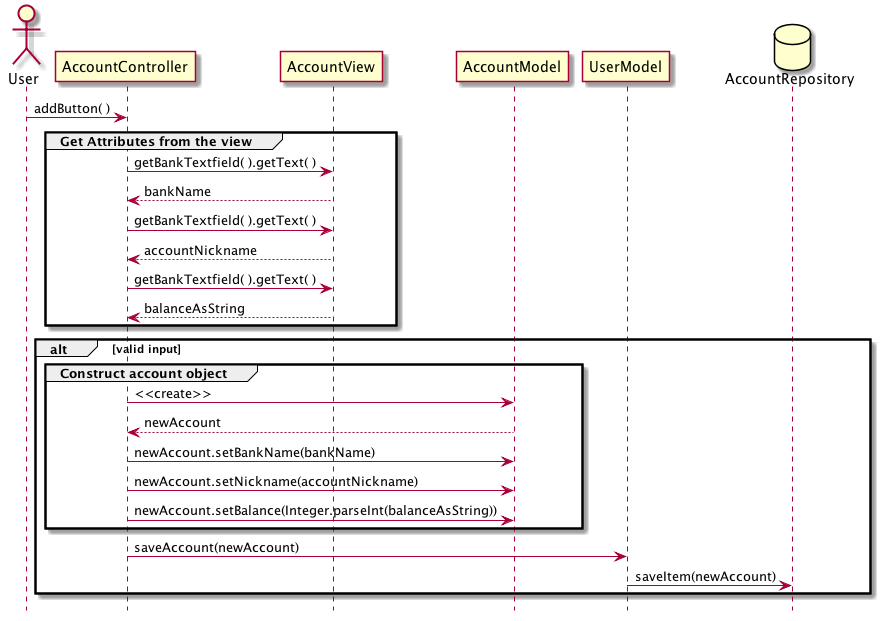
\includegraphics[width=\textwidth,height=\textheight,keepaspectratio]{diagrams/sequence/addAccount.png}
\captionof{figure}{Adding an account}

\newpage
\subsubsection{AccountRepository saving an account to the database}
When the saveItem method is called, the AccountRepository first creates an SQLValueMap (linked HashMap with keys and values of type String) to store the column-value mapping.

If the account is new (does not exist in the system), then the repository use the SQLStringFactory to build an insert query using the SQLValueMap, and execute it using updateSQL() from the Database class. The repository then updates the account's ID using the accountId returned from updateSQL() and adds the accounts to the repository's AccountMap.

If the account already exists, then the repository will construct a SQLValueMap for the where clause of the query using the account's ID. SQLStringFactory's is then used to generate a update query, which will be executed by calling the Database class's updateSQL() method. The returned accountId is unused.

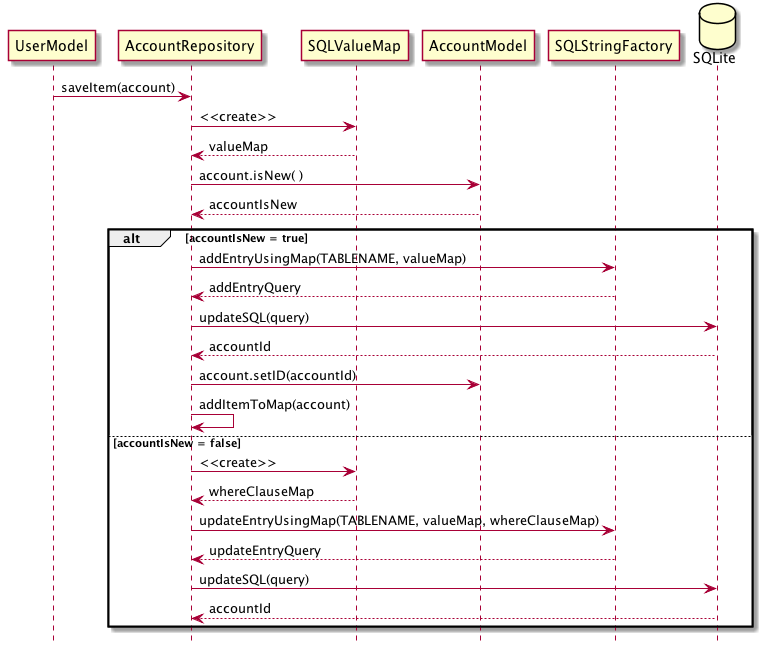
\includegraphics[width=\textwidth,height=\textheight,keepaspectratio]{diagrams/sequence/accRepoSaveItem.png}
\captionof{figure}{AccountRepository saving an account to the database}

\subsection{Adding a transaction}
After completing the text fields and pressing the "add" button, the addButton method from the TransactionController is triggered. The controller first gathers and validates the inputs. If the inputs are valid, the controller initializes an TransactionModel object and constructs it using setters. The controller then gets the AccountModel object from the UserModel, and uses its saveTransaction method. The AccountModel then calls its TransactionRepository's saveItem method.
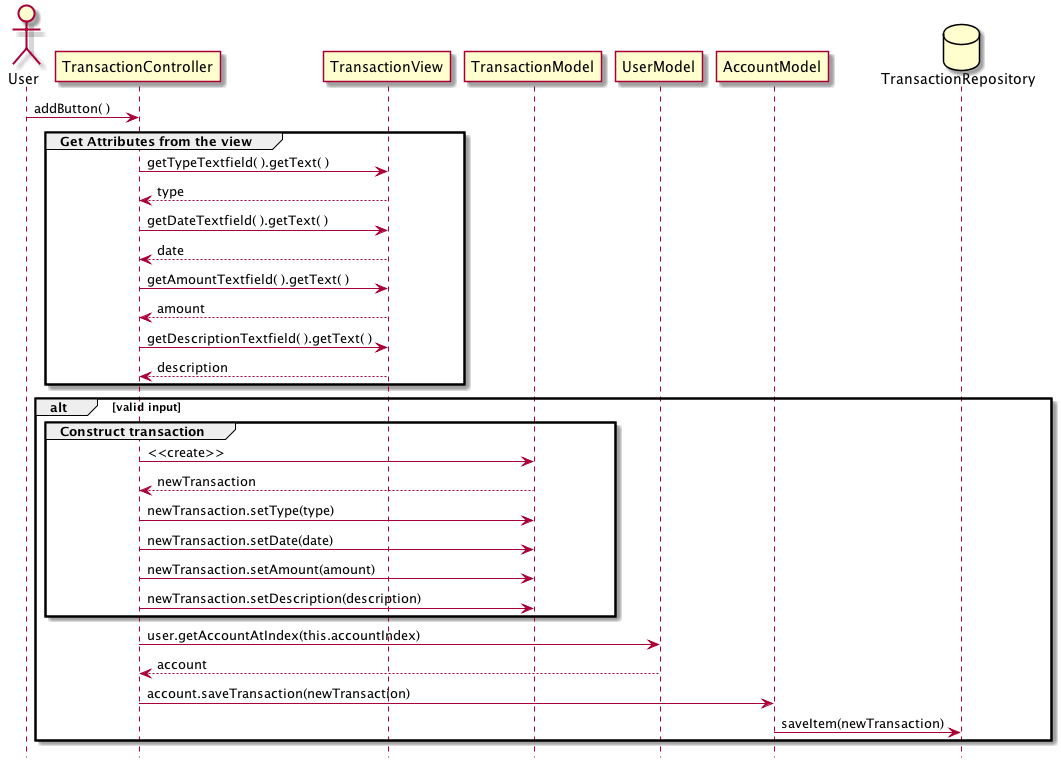
\includegraphics[width=\textwidth,height=\textheight,keepaspectratio]{diagrams/sequence/addTransaction.png}
\captionof{figure}{Adding a transaction}

\subsection{Importing a transaction}

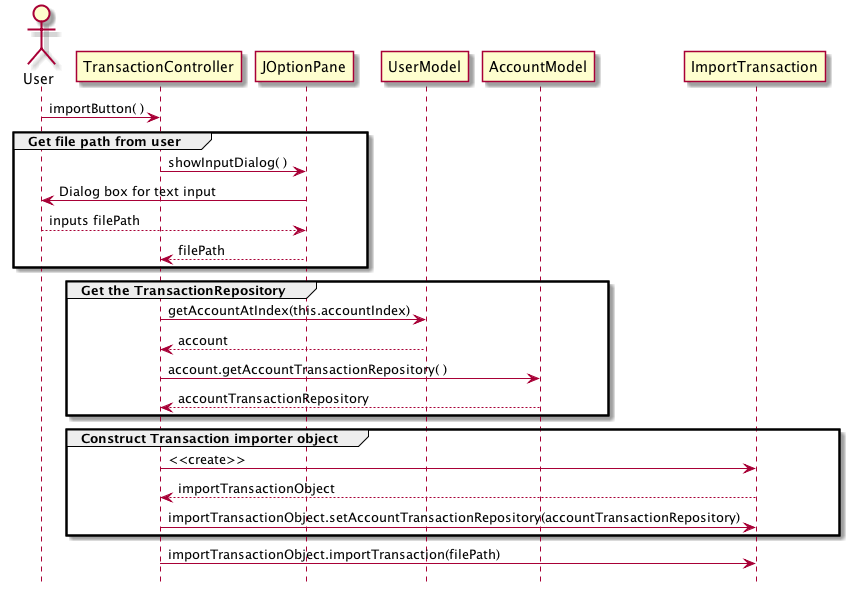
\includegraphics[width=\textwidth,height=\textheight,keepaspectratio]{diagrams/sequence/importTransaction.png}
\captionof{figure}{Importing a transaction}

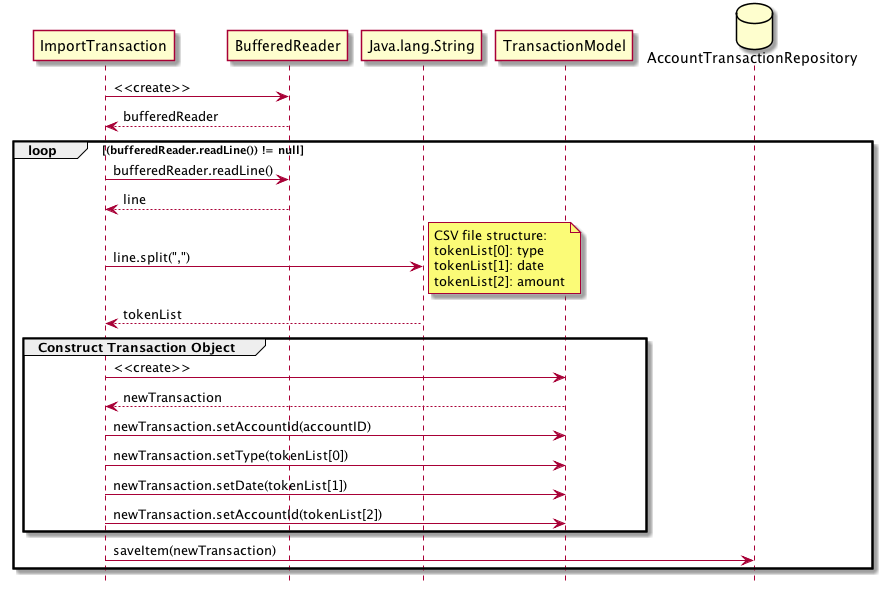
\includegraphics[width=\textwidth,height=\textheight,keepaspectratio]{diagrams/sequence/importTransaction2.png}
\captionof{figure}{Importing a transaction (cont.)}



\end{document}
